
\section{The multigrid preconditioned Krylov methods}
\label{sec:MGPre}

We concentrate on the system of discrete equations
\begin{equation}
  \label{eq:AX=B}
  \mA\mx=\mb,
\end{equation}

Matrix $\mA$ has right preconditioning as follows:
\begin{equation}
  \label{eq:RightPre}
  \mathbf{AK}^{-1}(\mathbf{Kx})=\mb.
\end{equation}
The preconditioned Krylov subspace methods are used for solving
\eqref{eq:RightPre}, such as BiCGSTAB and GMRES($m$).

\begin{alg}
  The GMRES($m$) algorithm with a right multigrid preconditioner
  appears as follows:

 \IncMargin{1em}
 \LinesNumbered
 \begin{algorithm}[H]
   \SetKwInOut{Precond}{Preconditions}
   \SetKwInOut{Postcond}{Postconditions}

   \caption{\texttt{GMRES($m,A,b,x,\epsilon$)}}
   \KwIn{$m\in\mathbb{Z}^+$, $A\in\mathbb{R}^{N\times N}$,
     $b\in\mathbb{R}^n$, $x\in\mathbb{R}^n$, 
     $\epsilon\in\mathbb{R}^+$.
     .}
   \KwOut{The solution which overwrites $x$.}
   \BlankLine
   Choose $x^{(0)}=x$, dimension $m$. matrix $\mathbf{H}=\mathbf{0}$
   with dim: $(m+1)\times m$\;
   $r^{(0)}=b-Ax^{(0)},\ \beta=\Vert r\Vert_2^2,\ f_1=r^{(0)}/\beta$\;
   \For{$j=1,\cdots,m$}{
     $u_j=K^{-1}f_j$\;
     $w=Au_j$\;
     \For{$i=1,\cdots,j$}{
       $h_{i,j}=(w,f_i)$\;
       $w = w - h_{i,j}f_j$\;
       $h_{j+1,j} = \Vert w \Vert_2$\;
       $f_{j+1} = w/h_{j+1,j}$\;
     }
   }
   Define $\mathbf{F}_m := [f_1,\cdots,f_m]$\;
   $x^{(m)}:=x^{(0)} + K^{-1}\mathbf{F}_my_m$ with $y_m=\min_y\Vert
   \beta e_1-\mathbf{H}y \Vert_2$\;
   Compute $r^{(m)}=b-Ax^{(m)}$\;
   \If{$\vert r^{(m)} \Vert_2 < \epsilon\Vert b \Vert_2$}{
     \textbf{Stop.}
   }\Else{
     restrart with $x^{(0)}\leftarrow x^{(m)}$\;
   }
 \end{algorithm}
 \DecMargin{1em}
 In line $4$, $K^{-1}f_j$ is the preconditioning step, which is one
 iteration of a multigrid cycle.
\end{alg}

The following theorem is an estimation of the convergence of
GMRES($m$) in cases where most of the eigenvalues (the last $n-l$
eigenvalues in the theorem below) of the preconditioned matrix
$\tilde{A}$ are close to $1\in\mathbb{C}.$

\begin{thm}
  \label{thm:GMRES}
  Let $\tilde{A}$ be an $n\times n$ nonsingular matrix with
  eigenvalues $\left\{\lambda_i\in\mathbb{C}\ |\  1\leq i \leq n\right\}$,
  $\overline{V}_l$ be the subspace spanned by the vectors
  $\left\{ v\ |\ \prod_{k>l}^n(\lambda_kI-\tilde{A})v=0\right\}$,
  $K_l$ be the Krylov subspave
  $K(l,r^{(0)},\tilde{A})=\mbox{span}\left\{ r^{(0)},
    \tilde{A}r^{(0)},\cdots, \tilde{A}^{l-1}r^{(0)}\right\}$, 
  $P_k$ be a set of $k$th-order complex polynomials $p_k(\lambda)$ that
  satisfy $p_k(0)=1$, and $r^{(0)}=b-\tilde{A}x^{(0)}$ be the initial
  residual. Define radius $\Gamma_i$ as
  \begin{equation}
    \label{eq:Radius}
    \Gamma_i := \max\left\{\Vert (\lambda_iI-\tilde{A})v \Vert_2\ |\ 
      v\in\overline{V}_{i-1}\cap K_i, \Vert v \Vert_2=1\right\}.
  \end{equation}
  Then a vector $\overline{r}^{(l)}$ defined by
  \begin{equation}
    \label{eq:rl}
    \overline{r}^{(l)} :=
    \left(\prod\limits_{i=1}^l\frac{1}{\lambda_i}(\lambda_iI-\tilde{A})\right)r^{(0)}
  \end{equation}
  is included in $\overline{V}_l\cap K_{l+1}.$

  Furthermore,
  \begin{equation}
    \label{eq:normOfrRl}
    \Vert \overline{r}^{(l)} \Vert_2 \leq
    \left(\prod\limits_{i=1}^l\frac{\Gamma_i}{|\lambda_i|}\right)
    \Vert r^{(0)}\Vert_2.
  \end{equation}
  Assuming $l<k\leq m$, then the norm of the residual of $k$th
  GMRES($m$) iteration can be estimated as follows:
  \begin{eqnarray}
    \label{eq:normOfResidual}
    \Vert r^{(k)} \Vert_2&\leq& \min\left\{\Vert
    p_{k-l}(\tilde{A})r^{(l)}\Vert_2 \ |\  p_{k-l}(\lambda)\in P_{k-l}\right\}
    \\
    \label{eq:normOfResidual2}
                         &\leq& \Vert (I-\tilde{A})^{k-l}\overline{r}^{(l)} \Vert_2.
  \end{eqnarray}
\end{thm}

According to Theorem \ref{thm:GMRES}, if some eigenvalues
$\lambda_i(i\leq l)$ are close to zero, the norm of
$\overline{r}^{(l)}$ becomes large. This suggests that we may need a
relatively large $k$ to reduce the residual by a certain order of
magnitude even if $l$ is not large.

Inequality \eqref{eq:normOfResidual} shows that $\Vert r^{(k)}
\Vert_2$ is not larger than the norm of the $(k-l)$th residual of
GMRES($m$) with initial residual $\overline{r}^{(l)}$ that is included
in the subspace corresponding to the eigenvalues close to one
$\left\{\lambda_i\ |\ i>l\right\}$.

Backtrack to the multigrid preconditioner, an iteration of a multigrid
cycle is equivalent to a Richardson iteration on  the preconditioned
matrix\cite{oosterlee_evaluation_1998}. With $K$ being the iteration
matrix, multigrid
can be written as follows:
\begin{equation}
  \label{eq:RichardsonIter}
  Kx^{(k+1)}+(A-K)x^{(k)}=b.
\end{equation}

If we use multigrid solver, the formulation is equivalent to
\begin{equation}
  \label{eq:Richardson2}
  x^{(k+1)} = x^{(k)} + K^{-1}(b-Ax^{(k)}) = x^{(k)}+K^{-1}r^{(k)};\
  r^{(k+1)} = (I-AK^{-1})r^{(k)}.
\end{equation}

The spectral radius of $I-AK^{-1}$ determines the convergence of
multigrid solver. With
this spectrum we can also investigate the convergence of
preconditioned GMRES method. From \eqref{eq:normOfResidual2}, the asymptotic
convergence of GMRES($m$) is at least faster than Richardson with an initial
residual. 

In \cite{oosterlee_evaluation_1998}, the author compared multigrid preconditioned
GMRES($m$) and multigrid solver in several singularly perturbed
problems. In \cite{guy_multigrid_2012}, the author compared multigrid
preconditioned GMRES($m$) and multigrid solver for implicit immersed
boundary equations. Here is an example:

\begin{exm}
  Here is a rotated anisotropic diffusion problem:
  \begin{equation}
    \label{eq:RotatingCon-D}
    -(\cos^2\beta +\epsilon\sin^2\beta)\frac{\partial^2\phi}{\partial
      x^2} - 2(\epsilon -
    1)\cos\beta\sin\beta\frac{\partial^2\phi}{\partial x\partial y} -
    (\epsilon\cos^2\beta + \sin^2\beta)\frac{\partial^2\phi}{\partial
      y^2} = 1
    \mbox{ on } \Omega=(0,1)\times (0,1).
\end{equation}
Here $\epsilon=10^{-5}$, $\beta=135^o$ and boundary conditions are prescribed :
\begin{equation}
  \begin{aligned}
    \pdfFrac{\phi}{n} = 0 \mbox{ on } \{x=0,\ 0\leq y\leq 1\},\{0\leq
    x\leq 1,\ y=0\},\\
    \phi=0\mbox{ on } \{x=1,\ 0\leq y\leq 1\},\{0\leq x\leq 1,\ y=1\}.
  \end{aligned}
\end{equation}

For this test problem, the eigenvalue spectrum of the Richardson
iteration matrix $I-AK^{-1}$ is investigated on a $33\times 33$ grid,
as presented in figure \ref{fig:spectrum}.

\begin{figure}[htbp]
      \centering
      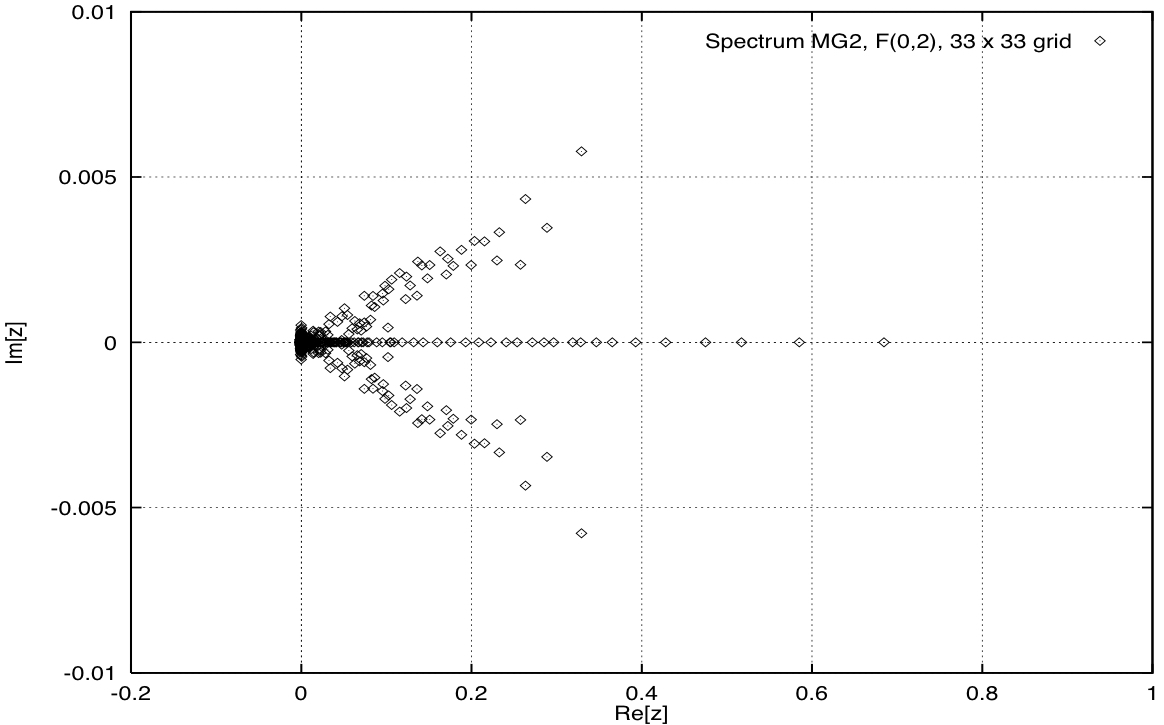
\includegraphics[width=0.5\textwidth]{Spectrum.png}
      \caption{The eigenvalue spectra for the rotated anisotropic
        diffusion problem,$\epsilon=10^{-5}$, $\beta=135^o$ on a
        $33\times 33$ grid.}
      \label{fig:spectrum}
    \end{figure}

It can be seen that the spectral radius for coarse grid problems is
already larger than 0.6. Therefore, the multigrid convergence slows
down more dramatically than the convergence of the preconditioned
Krylov methods. What's more, eigenvalues of the preconditioned matrix
$(AK^{-1})$ are clusted around $1$, which is advantageous for the
Krylov methods. The convergence of multigrid as solution methods and
as preconditioners for GMRES(20) is presented for $33\times 33$ grid
in Figure \ref{fig:convergence}.

\begin{figure}[htbp]
      \centering
      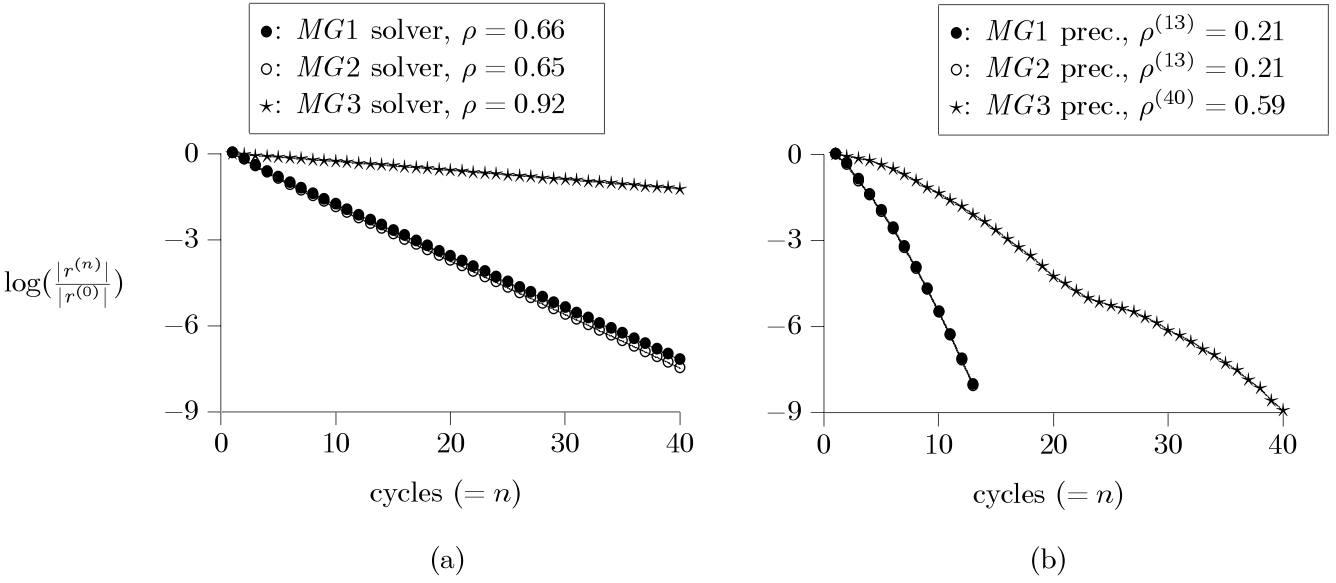
\includegraphics[width=0.75\textwidth]{Convergence.png}
      \caption{The convergence of the MG solvers (a), GMRES(20)
        with MG preconditioners (b) for the rotated anisotropic
        diffusion equation on a $33\times 33$ grid.}
      \label{fig:convergence}
    \end{figure}

MG1, MG2, MG3 are multigrid methods with different prolongation and
restriction operators. It can be seen that different prolongation and
restriction operators will affect the convergence rate. However, no
matter which operators are used, MG preconditioned GMRES($m$) method
performs better than MG solver in this problem.
\end{exm}



The conclusion is that the behaviors of the multigrid methods
are much more robust when they are used as preconditioners, problems
that could not be solved with the multigrid methods as solvers could
be solved with the preconditioned Krylov methods. The efficiency of
the multigrid solver alone is not impressive, but it is a very
effective preconditioner for Krylov methods. We also can improve the
preconditioned Krylov methods by using a more sophisticated smoother
in multigrid preconditioner, just like Figure \ref{fig:convergence}.

\section{Next step}
\label{sec:goal}

The follow-up work is mainly divided into two steps:

\begin{enumerate}
\item There is not much mathematical theory on multigrid
  preconditioned Krylov subspace methods, most papers do numerical
  experience to compare multigrid solver and multigrid preconditioner.
  So firstly we could investigate the eigenvalue spectrum of the
  Richardson iteration matrix $I-AK^{-1}$ in
  \eqref{eq:Richardson2} of three linear systems during solving GePuP
  equations. If many eigenvalues are clustered around zero and only a
  limited number of eigenvalues are far from zero, eigenvalues of the preconditioned
  matrix $AK^{-1}$  will be clustered around one, which is
  advantageous for the Krylov methods by Theorem \ref{thm:GMRES}.
\item Then implement multigrid preconditioned GMRES($m$) method,
  apply it to solve GePuP equations, and compare it with the original program
  in terms of convergence and efficiency.
\end{enumerate}



%%% Local Variables:
%%% mode: latex
%%% TeX-master: "MGPreconditioner_MathDoc"
%%% End:
